% TODO Escribir los comandos en negritas
\documentclass[a4paper,12pt]{article}
\usepackage[utf8]{inputenc}
\usepackage[T1]{fontenc}
% \usepackage[spanish]{babel}
\usepackage[colorlinks]{hyperref}
\usepackage{anysize}
\usepackage{minted}
\usepackage[most]{tcolorbox}
\definecolor{lightgreen}{rgb}{0.56, 0.93, 0.56}
\definecolor{moonstoneblue}{rgb}{0.45, 0.66, 0.76}
\hypersetup{urlcolor=cyan, linkcolor=black}
\marginsize{25mm}{25mm}{10mm}{25mm}
\linespread{1.2}

\title{Brief introduction to Python}
\author{Daniel Maldonado}
\date{February 2022}

\begin{document}
{\scshape\bfseries \maketitle}

\tableofcontents

\newpage
\section{Introduction}

\subsection{Why MedPCPy}

Within behavior analysis a common limiting factor is the inability to process data efficiently. Although given enough time most researchers would probably find ways to manage their data with varying degrees of success, many still struggle with manually converting their files to a more manageable format and making manual counts. Excel macros are a great tool for this, but they still require a great deal of involvement from the researcher, and given that they require human interaction they are prone to errors.

The motivation for making this library was to provide a free and accessible tool that allowed both new and seasoned researchers to quickly organize the data they need without spending  time learning to code. This tool aims to be easy to learn and use, less error prone than regular scripting, and above all, free (as in {\slshape gratis} and as in {\slshape libre}) for everyone. Med Associates\textsuperscript{\textregistered} provides their own software for a similar purpose, but it is prohibitively costly. Those who develop open tools share the belief that one cannot put a price neither on knowledge nor on the tools to produce it.

\subsection{About this package}

The team behind MedPCPy has extensively worked to make sure that the library works in all conditions. Bugs and special cases have been fixed to the best of our abilities. However---as is the case with anything programming-related---something could go wrong at some point. We encourage you to try and test the library in different cases, and to let us know when things go wrong so that we can improve the library and make it more useful for everyone.

If you find that something does not work as expected, or if you have any ideas on how to improve the library, please feel free to either open an issue on the project's \href{https://github.com/JuodaanViinaa/Laboratorio}{GitHub} page, or \href{mailto:maldonadodaniel96@outlook.com}{email us}.

\newpage
\section{Brief introduction to Python}

Python is a general purpose, interpreted programming language. Although it is not as fast as other languages, such as $C$, its simple syntax makes it ideal for purposes as machine learning and artificial intelligence, among many others. It is easy to learn and very powerful. For those reasons it was chosen to develop this library.

\subsection{Installing Python}

Python can be installed on any machine by downloading it from its \href{https://www.python.org/}{official page}, from the Microsoft Store, or from any Linux repository. Several tutorials on YouTube will be of help if any problems arise during the installation.

\subsection{Integrated Development Environments}

For beginner users and those who wish a working ready-to-use experience, several IDEs are available. An IDE is a program which provides services to facilitate computer programming, such as syntax highlighting, code autocompletion, easy documentation access, and more. We recommend the community edition of \href{https://www.jetbrains.com/pycharm/download/}{PyCharm} because it is free and can automatically manage virtual environments. Other common IDEs are \href{https://www.spyder-ide.org/}{Spyder}, and \href{https://code.visualstudio.com/}{Visual Studio Code}. However, any IDE or text editor will be more than enough.

\subsection{Virtual Environments}

Python is a modular language. Any number of third-party libraries can be installed on a system. This allows the use of an unlimited amount of tools created by the community for all sorts of tasks. That, however, can give rise to conflicts if, for example, a project in which someone is working requires version 2 of a library, but a different project requires version 3. In order to solve this issue, as of Python 3.3 the {\slshape virtualenv} module is included with every standard Python installation.

The {\slshape virtualenv} module allows the creation of {\itshape virtual environments}: containers isolated from the system-wide install which have their own Python executable and can have their independent set of installed Python packages. These packages are accessible only from within the virtual environment, and thus avoid version conflicts as long as projects with different version requirements are hosted in their own separate environments.

The creation of virtual environments is simple. And in fact the PyCharm IDE makes it almost automatic. To create a virtual environment in PyCharm one needs only to select the ``New Project'' button, choose a directory in which to create it, select ``New environment using: Virtualenv'', and then click on ``Create'':

\begin{figure}[!ht]
    \begin{center}
        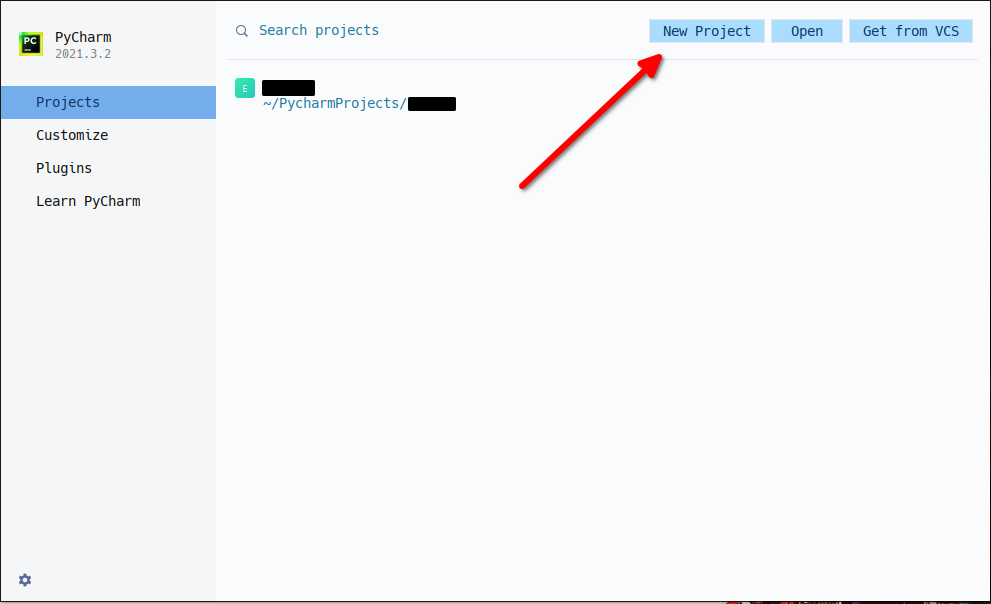
\includegraphics[scale=0.5]{pycharm-new-project.png}
    \end{center}
\end{figure}

\begin{figure}[!ht]
    \begin{center}
        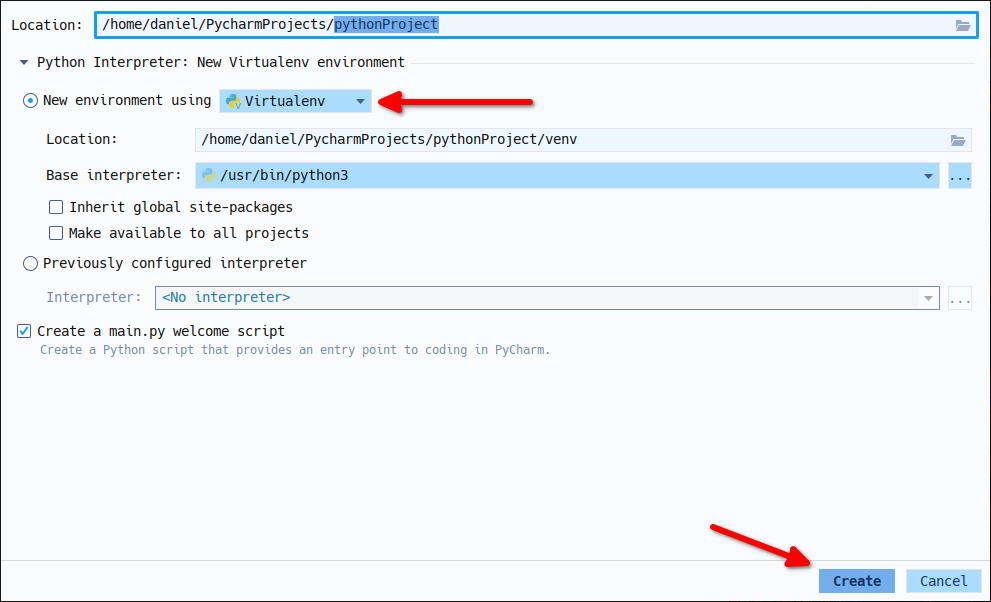
\includegraphics[scale=0.5]{pycharm-create.png}
    \end{center}
\end{figure}

To create a virtual environment without an IDE it is necessary to use the terminal or command line. On windows it can be accessed by pressing WindowsKey + R, and writing "cmd" on the prompt. Clicking "Ok" will then open the terminal.

On Mac, the terminal can be opened by clicking on the Launchpad icon, typing "terminal" and clicking on the Terminal program.

On Linux, I trust you.

Once the terminal is open, a virtual environment can be created by running the command
\begin{tcolorbox}[
    enhanced,
    attach boxed title to top left={xshift=6mm,yshift=-3mm},
    colback=lightgreen!20,
    colframe=lightgreen,
    colbacktitle=lightgreen,
    sharp corners,
    ]
    \begin{minted}{fish}
python -m venv [directory]
    \end{minted}
\end{tcolorbox}
\noindent where [directory] is the path to the directory in which you will create the environment. After the virtual environment is created, it can be activated by running a script installed by venv. On windows, this is done with
\begin{tcolorbox}[
    enhanced,
    attach boxed title to top left={xshift=6mm,yshift=-3mm},
    colback=lightgreen!20,
    colframe=lightgreen,
    colbacktitle=lightgreen,
    sharp corners,
    ]
    \begin{minted}{text}
myenv\Scripts\activate.bat
    \end{minted}
\end{tcolorbox}
\noindent on either Mac or Linux this is done with
\begin{tcolorbox}[
    enhanced,
    attach boxed title to top left={xshift=6mm,yshift=-3mm},
    colback=lightgreen!20,
    colframe=lightgreen,
    colbacktitle=lightgreen,
    sharp corners,
    ]
    \begin{minted}{text}
source myenv/bin/activate
    \end{minted}
\end{tcolorbox}
\noindent where ``myenv'' is the name of the virtual environment directory just created.

After the environment is activated, any packages that are installed will only be so in the local environment. Python scripts that are run while inside the environment will be able to use any packages installed in it.

To deactivate or exit a virtual environment one only needs to run ``deactivate'' in the terminal. PyCharm automatically opens and closes virtual environments when opening and closing projects.

\subsection{Python basics}

Providing an introductory course to Python is not the purpose of this guide. However, aiming to be as accessible as possible, the very basics needed to understand and use the MedPCPy library will be explained.

\subsubsection{Data types}

Several data types are available in Python. The most common ones are \verb|strings|, \verb|integers|, \verb|floats|, \verb|lists|, \verb|tuples|, \verb|dictionaries|, and \verb|booleans|.

\vspace{5mm}
\noindent\begin{tabular}{|c|c|c|c|}
    \hline
    {\bfseries Name}&{\bfseries Type}&{\bfseries Description}&{\bfseries Examples}\\
    \hline
    Strings&str&Ordered sequence of characters&"Hello, world"\ \ \ "123"\\
    \hline
    Integers&int&Whole numbers&0\ \ \ 399\ \ \ 1996\\
    \hline
    Floating points&float&Numbers with a decimal point&0.0\ \ \ 3.1415\\
    \hline
    Lists&list&Ordered sequence of objects&[1, 3.6, "one"]\\
    \hline
    Tuples&tup&Non-modifiable list&(10, "hello", 1.4)\\
    \hline
    Dictionaries&dict&Ordered Key:Value pairs&\{"name": "Giorno", "age": 15\}\\
    \hline
    Boolean&bool&Logical \verb|True|/\verb|False| values&\verb|True|\ \ \ \verb|False|\\
    \hline
\end{tabular}

\vspace{5mm}
\subsubsection{Variable assignment}

All data types can be assigned to variables to make them more manageable.

\begin{tcolorbox}[
    enhanced,
    attach boxed title to top left={xshift=6mm,yshift=-3mm},
    colback=lightgreen!20,
    colframe=lightgreen,
    colbacktitle=lightgreen,
    title=Python,
    fonttitle=\bfseries\color{black},
    boxed title style={size=small,colframe=lightgreen,sharp corners},
    sharp corners,
    ]
    \begin{minted}[linenos]{python}
my_string = "Hello, world!"
my_int = 745
my_float = 100.0
my_list = [my_string, my_int, my_float]
my_tuple = (my_string, my_int, my_float, my_list)
my_dict = {
    "name": "Joseph",
    "nationality": "english",
    "age": 18
}
my_bool = True
    \end{minted}
\end{tcolorbox}

As you can see, having named variables instead of crude data is more readable. It also allows the use of a previously declared variable on the declaration of another one.

\subsubsection{Nesting}

Lists, tuples, and dictionaries allow nesting other lists, tuples or dictionaries within them with no limit to how deep the nesting can go.

\begin{tcolorbox}[
    enhanced,
    attach boxed title to top left={xshift=6mm,yshift=-3mm},
    colback=lightgreen!20,
    colframe=lightgreen,
    colbacktitle=lightgreen,
    title=Python,
    fonttitle=\bfseries\color{black},
    boxed title style={size=small,colframe=lightgreen,sharp corners},
    sharp corners,
    ]
    \begin{minted}[linenos]{python}
list_1 = [1, 2, 3, 4]
list_2 = [5, 6, 7, 8]
super_list = [list_1, list_2]
    \end{minted}
\end{tcolorbox}

In this example the variable \verb|super_list| would contain two items, both of which would be lists. I.e., the code above is equivalent to:

\begin{tcolorbox}[
    enhanced,
    attach boxed title to top left={xshift=6mm,yshift=-3mm},
    colback=lightgreen!20,
    colframe=lightgreen,
    colbacktitle=lightgreen,
    title=Python,
    fonttitle=\bfseries\color{black},
    boxed title style={size=small,colframe=lightgreen,sharp corners},
    sharp corners,
    ]
    \begin{minted}[linenos]{python}
super_list = [[1, 2, 3, 4], [5, 6, 7, 8]]
    \end{minted}
\end{tcolorbox}

And the same is true for either tuples or dictionaries:

\begin{tcolorbox}[
    enhanced,
    attach boxed title to top left={xshift=6mm,yshift=-3mm},
    colback=lightgreen!20,
    colframe=lightgreen,
    colbacktitle=lightgreen,
    title=Python,
    fonttitle=\bfseries\color{black},
    boxed title style={size=small,colframe=lightgreen,sharp corners},
    sharp corners,
    ]
    \begin{minted}[linenos]{python}
super_tuple = (("a", "b", "c"), "d")
dictionary = {
    "names": ["Jonathan", "Joseph", "Giorno"],
    "nationalities": ["english", "american", "italian"]
}
    \end{minted}
\end{tcolorbox}

This is also not limited to the same type of variable. That is, lists can contain tuples and dictionaries, tuples can contain lists and dictionaries, and so on.

Dictionaries can even be nested inside other dictionaries:

\begin{tcolorbox}[
    enhanced,
    attach boxed title to top left={xshift=6mm,yshift=-3mm},
    colback=lightgreen!20,
    colframe=lightgreen,
    colbacktitle=lightgreen,
    title=Python,
    fonttitle=\bfseries\color{black},
    boxed title style={size=small,colframe=lightgreen,sharp corners},
    sharp corners,
    ]
    \begin{minted}[linenos]{python}
planets = {
    "earth": {"color": "blue", "population": "lots"},
    "mars": {"color": "red", "population": "none"}
}
    \end{minted}
\end{tcolorbox}

The analysis list used in the {\scshape MedPCPy} library is a list comprised of dictionaries with other, nested dictionaries:

\begin{tcolorbox}[
    enhanced,
    attach boxed title to top left={xshift=6mm,yshift=-3mm},
    colback=lightgreen!20,
    colframe=lightgreen,
    colbacktitle=lightgreen,
    title=Python,
    fonttitle=\bfseries\color{black},
    boxed title style={size=small,colframe=lightgreen,sharp corners},
    sharp corners,
    ]
    \begin{minted}[linenos]{python}
analysis_list = [
    # Measure 1
    {"fetch": {"cell_row": 1,
               "cell_column": 1,
               "sheet": "Measure1",
               "summary_column_dict": measure1_cols,
               "offset": 0,
               }},
               ...
                ]
    \end{minted}
\end{tcolorbox}

Be mindful that the use of space in the declaration of lists, tuples or dictionaries has no syntactic purpose. The distribution is only to increase readability.

\subsubsection{Functions}

Functions are blocks of reusable code which perform actions that are needed frequently. They are declared only once but can be executed any time they are called. They help increase the readability and modularity of code.

Functions are declared with the \verb|def| keyword, followed by the name which the user desires to assign to it, optionally the arguments in parentheses, and a semicolon. They can either only perform an action, or return a value which can then be assigned to a variable.

\begin{tcolorbox}[
    enhanced,
    attach boxed title to top left={xshift=6mm,yshift=-3mm},
    colback=lightgreen!20,
    colframe=lightgreen,
    colbacktitle=lightgreen,
    title=Python,
    fonttitle=\bfseries\color{black},
    boxed title style={size=small,colframe=lightgreen,sharp corners},
    sharp corners,
    ]
    \begin{minted}[linenos]{python}
def hello_function():
    print("Pizza Mozzarella")

def my_sum_function(a, b):
    return a + b
    \end{minted}
\end{tcolorbox}

Then they are called with their name and the necessary arguments:

\begin{tcolorbox}[
    enhanced,
    attach boxed title to top left={xshift=6mm,yshift=-3mm},
    colback=lightgreen!20,
    colframe=lightgreen,
    colbacktitle=lightgreen,
    title=Python,
    fonttitle=\bfseries\color{black},
    boxed title style={size=small,colframe=lightgreen,sharp corners},
    sharp corners,
    ]
    \begin{minted}[linenos]{python}
hello_function()

x = 20
y = 30
result = my_sum_function(x, y)
print(result)
    \end{minted}
\end{tcolorbox}

This would result in printing the string \verb|"Pizza Mozzarella"|, assigning the value \verb|50| to the \verb|result| variable, and then printing that variable as well:

\begin{tcolorbox}[
    enhanced,
    attach boxed title to top left={xshift=6mm,yshift=-3mm},
    colback=lightgray!20,
    colframe=lightgray,
    colbacktitle=lightgray,
    title=Output,
    fonttitle=\bfseries\color{black},
    boxed title style={size=small,colframe=lightgray,sharp corners},
    sharp corners,
    ]
    \begin{minted}{text}
Pizza Mozzarella
50
    \end{minted}
\end{tcolorbox}

Functions can have positional arguments (identified by their position) and keyword arguments (identified by a keyword). Additionally, if a default value for an argument is provided when the function is defined, then that argument becomes optional and, if it is not declared when the function is called, it will take the default value.

\begin{tcolorbox}[
    enhanced,
    attach boxed title to top left={xshift=6mm,yshift=-3mm},
    colback=lightgreen!20,
    colframe=lightgreen,
    colbacktitle=lightgreen,
    title=Python,
    fonttitle=\bfseries\color{black},
    boxed title style={size=small,colframe=lightgreen,sharp corners},
    sharp corners,
    ]
    \begin{minted}[linenos]{python}
def another_function(name = "Ford Prefect"):
    print(f"Hello, my name is {name}")

another_function("Arthur Dent")
another_function()
    \end{minted}
\end{tcolorbox}

This would print the following:

\begin{tcolorbox}[
    enhanced,
    attach boxed title to top left={xshift=6mm,yshift=-3mm},
    colback=lightgray!20,
    colframe=lightgray,
    colbacktitle=lightgray,
    title=Output,
    fonttitle=\bfseries\color{black},
    boxed title style={size=small,colframe=lightgray,sharp corners},
    sharp corners,
    ]
    \begin{minted}{text}
Hello, my name is Arthur Dent
Hello, my name is Ford Prefect
    \end{minted}
\end{tcolorbox}
Given that the optional argument \verb|name| took the default value \verb|Ford Prefect| on the second calling of the function.

\subsubsection{Classes and objects}

Python is an object-oriented programming language, which means that a good deal of its functionality is built around ``objects'' which contain data and code. In object-oriented programming the code is organized into reusable ``blueprints'' called \verb|classes|, and those classes can be used to create individual instances of \verb|objects|, which share the general structure of the class, but have their own particular content. Objects can have properties (data) and methods (functions) associated to them.

A class is declared with the \verb|class| keyword, the name of the class, and a semicolon. Class attributes are declared in a special function called \verb|__init__|, and methods associated with the class are declared as functions inside of it.

\begin{tcolorbox}[
    enhanced,
    attach boxed title to top left={xshift=6mm,yshift=-3mm},
    colback=lightgreen!20,
    colframe=lightgreen,
    colbacktitle=lightgreen,
    title=Python,
    fonttitle=\bfseries\color{black},
    boxed title style={size=small,colframe=lightgreen,sharp corners},
    sharp corners,
    ]
    \begin{minted}[linenos]{python}
class Dog:
    def __init__(name, age):
        self.dog_name = name
        self.dog_age = age

    def print_name():
        print(f"""
        Hello, my name is {self.dog_name},
        and I am {self.dog_age} years old. Woof!
        """)
    \end{minted}
\end{tcolorbox}

Afterwards, the class can be used as a blueprint to create individual objects with the general properties of the class.

\begin{tcolorbox}[
    enhanced,
    attach boxed title to top left={xshift=6mm,yshift=-3mm},
    colback=lightgreen!20,
    colframe=lightgreen,
    colbacktitle=lightgreen,
    title=Python,
    fonttitle=\bfseries\color{black},
    boxed title style={size=small,colframe=lightgreen,sharp corners},
    sharp corners,
    ]
    \begin{minted}[linenos]{python}
my_dog = Dog("John", 5)
    \end{minted}
\end{tcolorbox}

The creation of the object is similar to the calling of a function. In this example the end result would be an object of class \verb|Dog| being assigned to the variable \verb|my_dog|. This object would have two attributes and a method associated. The attributes can be changed with the notation \verb|object.attribute = [new value]|.

\begin{tcolorbox}[
    enhanced,
    attach boxed title to top left={xshift=6mm,yshift=-3mm},
    colback=lightgreen!20,
    colframe=lightgreen,
    colbacktitle=lightgreen,
    title=Python,
    fonttitle=\bfseries\color{black},
    boxed title style={size=small,colframe=lightgreen,sharp corners},
    sharp corners,
    ]
    \begin{minted}[linenos]{python}
my_dog.dog_name = "Cat"
    \end{minted}
\end{tcolorbox}

And the method can be used with the notation \verb|object.method()|.

\begin{tcolorbox}[
    enhanced,
    attach boxed title to top left={xshift=6mm,yshift=-3mm},
    colback=lightgreen!20,
    colframe=lightgreen,
    colbacktitle=lightgreen,
    title=Python,
    fonttitle=\bfseries\color{black},
    boxed title style={size=small,colframe=lightgreen,sharp corners},
    sharp corners,
    ]
    \begin{minted}[linenos]{python}
my_dog.print_name()
    \end{minted}
\end{tcolorbox}

This would result in printing the phrase

\begin{tcolorbox}[
    enhanced,
    attach boxed title to top left={xshift=6mm,yshift=-3mm},
    colback=lightgray!20,
    colframe=lightgray,
    colbacktitle=lightgray,
    title=Output,
    fonttitle=\bfseries\color{black},
    boxed title style={size=small,colframe=lightgray,sharp corners},
    sharp corners,
    ]
    \begin{minted}{text}
Hello, my name is Cat,
and I am 5 years old. Woof!
    \end{minted}
\end{tcolorbox}

The core of the MedPCPy library is an object of a particular class called \verb|Analyzer|. It has methods to get the sessions associated with a subject, convert files to .xlsx format, create documents, and compute the appropriate responses and latencies.

\subsubsection{Installing libraries}

Python is a modular language, which means that its functionality can be extended by including code created by the community. This code is shared through libraries which users can easily install into their system and import into their projects.

From within the virtual environment libraries can be installed by running the command

\begin{tcolorbox}[
    enhanced,
    attach boxed title to top left={xshift=6mm,yshift=-3mm},
    colback=lightgreen!20,
    colframe=lightgreen,
    sharp corners,
    ]
    \begin{minted}{text}
pip install [library-name]
    \end{minted}
\end{tcolorbox}
\noindent on the terminal. PyCharm can handle the installation of libraries in a longer but more intuitive way if one is not accustomed to working in the terminal. To install a new library navigate to \verb|File| \textrightarrow \verb|Settings| \textrightarrow \verb|Project| \textrightarrow \verb|Python interpreter|. There, click on the + symbol, type the name of the library you wish to install, and click ``Install''.

\begin{figure}[!ht]
    \begin{center}
        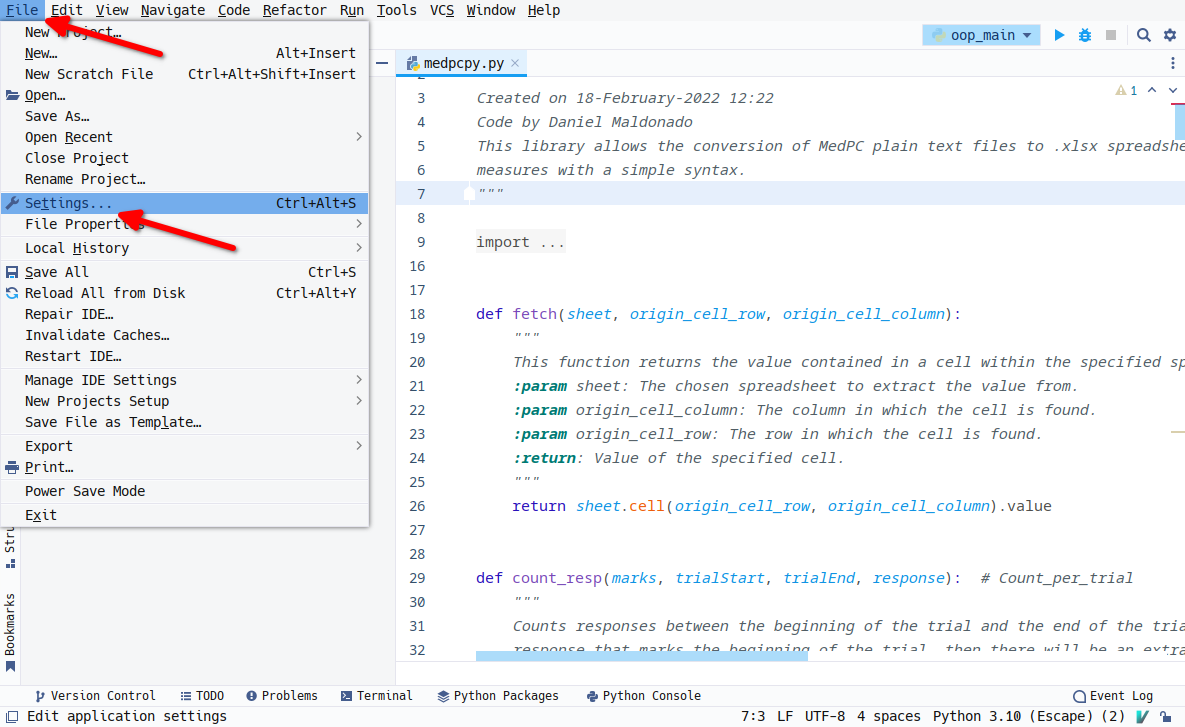
\includegraphics[scale=0.4]{pycharm-settings.png}
    \end{center}
\end{figure}

\begin{figure}[!ht]
    \begin{center}
        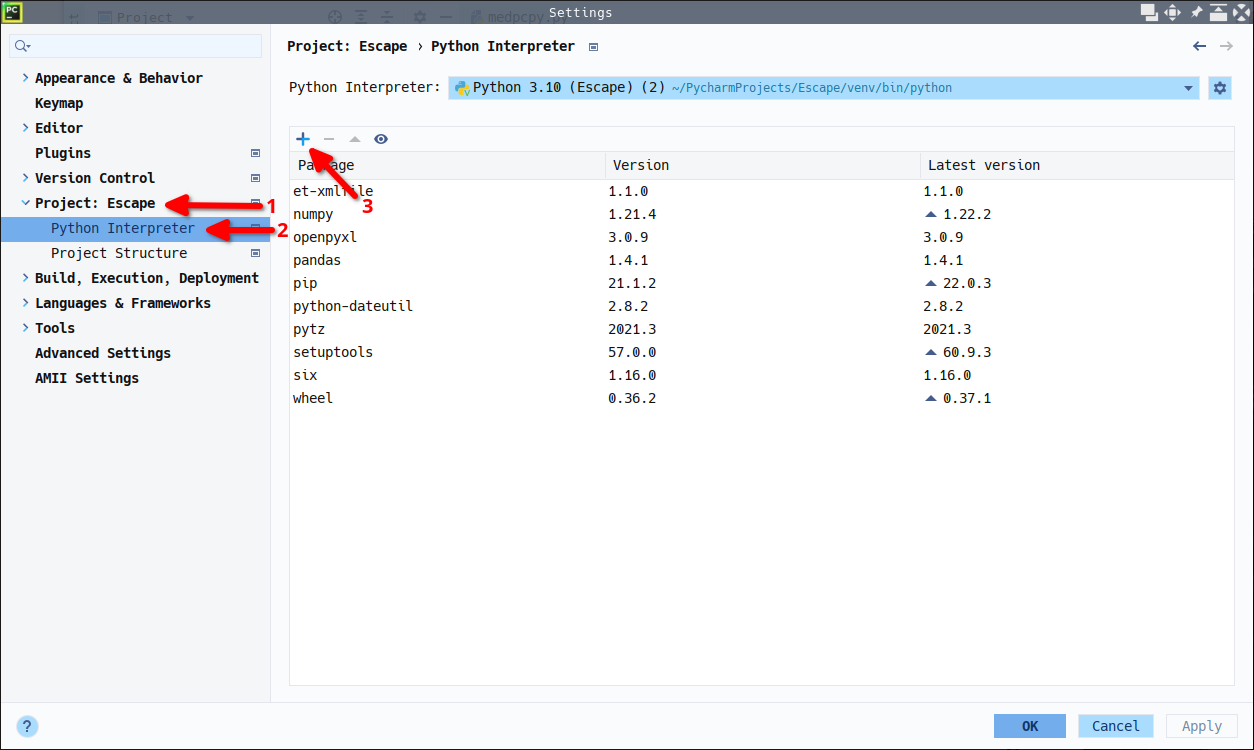
\includegraphics[scale=0.4]{pycharm-interpreter-settings.png}
    \end{center}
\end{figure}

\begin{figure}[!ht]
    \begin{center}
        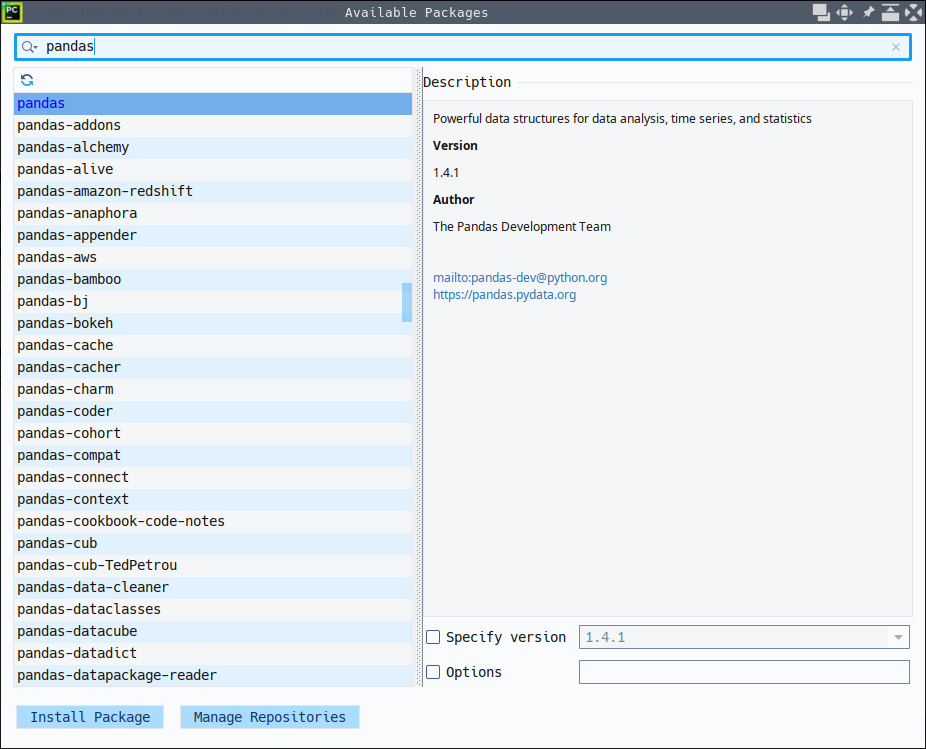
\includegraphics[scale=0.4]{pycharm-library-install.png}
    \end{center}
\end{figure}

\newpage
\ 
\newpage
\section{This library}

To install this library run the command

\begin{tcolorbox}[
    enhanced,
    attach boxed title to top left={xshift=6mm,yshift=-3mm},
    colback=lightgreen!20,
    colframe=lightgreen,
    sharp corners,
    ]
    \begin{minted}{text}
pip install medpcpy
    \end{minted}
\end{tcolorbox}

\noindent on the terminal, or install it from the interface of your IDE of choice. It will install all its required dependencies by default.

\subsection{First steps}

The first thing to do is to check that your system is ready to begin the process of file conversion and data extraction. To do this, you must create three separate folders in any part of your system that you desire. These folders will contain the raw files before the analysis (TemporaryDir), the raw files after the analysis (PermanentDir), and the already converted and processed .xlsx files (ConvertedDir). The reason why two separate folders for raw files are needed is that the library scans the temporary folder and uses its contents to determine the names of the subjects with at least one associated file and the numbers of the sessions to analyze. If all files are contained in the temporary folder, then all files will be processed every time the script is run. That is the reason why only new, unprocessed files must be placed in the temporary folder. It is worth noting that the directory names are arbitrary.

\begin{figure}[!ht]
    \begin{center}
        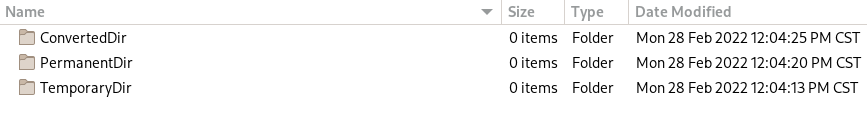
\includegraphics[scale=0.7]{directories.png}
    \end{center}
\end{figure}

Then, you must check that your files' names follow the format

\begin{tcolorbox}[
    enhanced,
    attach boxed title to top left={xshift=6mm,yshift=-3mm},
    colback=lightgreen!20,
    colframe=lightgreen,
    sharp corners,
    ]
    \begin{minted}{text}
[subject name][separator][session number]
    \end{minted}
\end{tcolorbox}
\noindent to guarantee that the library is able to read them. The \verb|separator| is a character or group of characters that, as you can guess, separates the subject name and session number. It can be any character or group of characters, but there must be a separator. For example, if the files were named \verb|"Subject_1_session_1"|, \verb|"Subject_1_session_2"|, etc., the \verb|separator| would be \verb|"_session_"|, since that is what is placed between the subject name and the session number. More specifically, \verb|"Subject_1"| would be the subject name, \verb|"_session_"| would be the separator, and \verb|"1"| would be the session number.

\subsection{Importing the library}

The MedPCPy library can be imported to the current working script with the line

\begin{tcolorbox}[
    enhanced,
    attach boxed title to top left={xshift=6mm,yshift=-3mm},
    colback=lightgreen!20,
    colframe=lightgreen,
    colbacktitle=lightgreen,
    title=Python,
    fonttitle=\bfseries\color{black},
    boxed title style={size=small,colframe=lightgreen,sharp corners},
    sharp corners,
    ]
    \begin{minted}[linenos]{python}
from medpcpy import *
    \end{minted}
\end{tcolorbox}

The star \verb|"*"| makes all the functions and classes available to the current project without the need to write the name of the library every time they are used.

\subsection{Declaring variables}

Several variables have to be declared before the \verb|Analyzer| object. These are the summary file name, directory paths, subject names, column dictionaries, sheet names, and the analysis list. A full explanation of their requirements (particularly for the column dictionaries and the analysis list, whose names are less intuitive) is provided in the \href{https://github.com/JuodaanViinaa/Laboratorio/blob/translate/README.md}{readme} file of the GitHub \href{https://github.com/JuodaanViinaa/Laboratorio/tree/translate}{repository}. Here only an example declaration is provided:

\begin{tcolorbox}[
    enhanced,
    attach boxed title to top left={xshift=6mm,yshift=-3mm},
    colback=lightgreen!20,
    colframe=lightgreen,
    colbacktitle=lightgreen,
    title=Python,
    fonttitle=\bfseries\color{black},
    boxed title style={size=small,colframe=lightgreen,sharp corners},
    sharp corners,
    ]
    \begin{minted}[linenos]{python}
file = "your_summary_filename.xlsx"
temp_directory = "/path/to/your/temporary/directory/"
perm_directory = "/path/to/your/permanent/raw/directory/"
conv_directory = "/path/to/your/converted/directory/"
subjects = ["Subject1", "Subject2", "Subject3"]
measure1_cols = {"Subject1": 2, "Subject2": 4, "Subject3": 6}
sheets = ["Measure1"]

analysis_list = [
    # Measure 1
    {"fetch": {"cell_row": 1,
               "cell_column": 1,
               "sheet": "Measure1",
               "summary_column_dict": measure1_cols,
               "offset": 0,
               }},
    ]
    \end{minted}
\end{tcolorbox}

After that, the \verb|Analyzer| object can be declared, though it wont yet be ready to analyze data.

\begin{tcolorbox}[
    enhanced,
    attach boxed title to top left={xshift=6mm,yshift=-3mm},
    colback=lightgreen!20,
    colframe=lightgreen,
    colbacktitle=lightgreen,
    title=Python,
    fonttitle=\bfseries\color{black},
    boxed title style={size=small,colframe=lightgreen,sharp corners},
    sharp corners,
    ]
    \begin{minted}[linenos]{python}
my_analyzer = Analyzer(fileName=file,
                temporaryDirectory=temp_directory,
                permanentDirectory=perm_directory,
                convertedDirectory=conv_directory
                subjectList=subjects, suffix="_",
                sheets=sheets,
                analysisList=analysis_list,
                relocate=False)
    \end{minted}
\end{tcolorbox}

After its declaration, the \verb|Analyzer| object must be used to convert at least one file to .xlsx format with the \verb|.convert()| method.

\begin{tcolorbox}[
    enhanced,
    attach boxed title to top left={xshift=6mm,yshift=-3mm},
    colback=lightgreen!20,
    colframe=lightgreen,
    colbacktitle=lightgreen,
    title=Python,
    fonttitle=\bfseries\color{black},
    boxed title style={size=small,colframe=lightgreen,sharp corners},
    sharp corners,
    ]
    \begin{minted}[linenos]{python}
my_analyzer.convert()
    \end{minted}
\end{tcolorbox}

Then, any one of the converted files must be manually inspected in order to determine the columns in which both the time and the marks (explained in the \href{https://github.com/JuodaanViinaa/Laboratorio/blob/translate/README.md}{readme} file) are located. Each mark is associated with a particular time of occurrence since the beginning of the session. They are assumed to be written on a Med array with the format ``{\scshape time.mark}'', and after conversion they are written on two adjacent columns of the same length. 

After that, the \verb|Analyzer| object can be fully declared with the mark and time columns, and is now ready to analyze data.

\begin{tcolorbox}[
    enhanced,
    attach boxed title to top left={xshift=6mm,yshift=-3mm},
    colback=lightgreen!20,
    colframe=lightgreen,
    colbacktitle=lightgreen,
    title=Python,
    fonttitle=\bfseries\color{black},
    boxed title style={size=small,colframe=lightgreen,sharp corners},
    sharp corners,
    ]
    \begin{minted}[linenos]{python}
my_analyzer = Analyzer(fileName=file,
                temporaryDirectory=temp_directory,
                permanentDirectory=perm_directory,
                convertedDirectory=conv_directory
                subjectList=subjects, suffix="_",
                sheets=sheets,
                analysisList=analysis_list,
                timeColumn="O",
                markColumn="P",
                relocate=False)
    \end{minted}
\end{tcolorbox}

\subsection{Final use}

After the \verb|Analyzer| object is declared with all its relevant variables, the analysis of an arbitrary number of sessions and subjects can be done with a single click.  The analysis is called with the \verb|.complete_analysis()| method:
\begin{tcolorbox}[
    enhanced,
    attach boxed title to top left={xshift=6mm,yshift=-3mm},
    colback=lightgreen!20,
    colframe=lightgreen,
    colbacktitle=lightgreen,
    title=Python,
    fonttitle=\bfseries\color{black},
    boxed title style={size=small,colframe=lightgreen,sharp corners},
    sharp corners,
    ]
    \begin{minted}[linenos]{python}
my_analyzer.complete_analysis()
    \end{minted}
\end{tcolorbox}

To run the analysis the user only needs to place their files on the temporary directory and run the script. This can be done by going to the ``Run'' menu and clicking on ``Run [name of your script]'' or by pressing \verb|Shift + F10|.

\begin{figure}[!ht]
    \begin{center}
        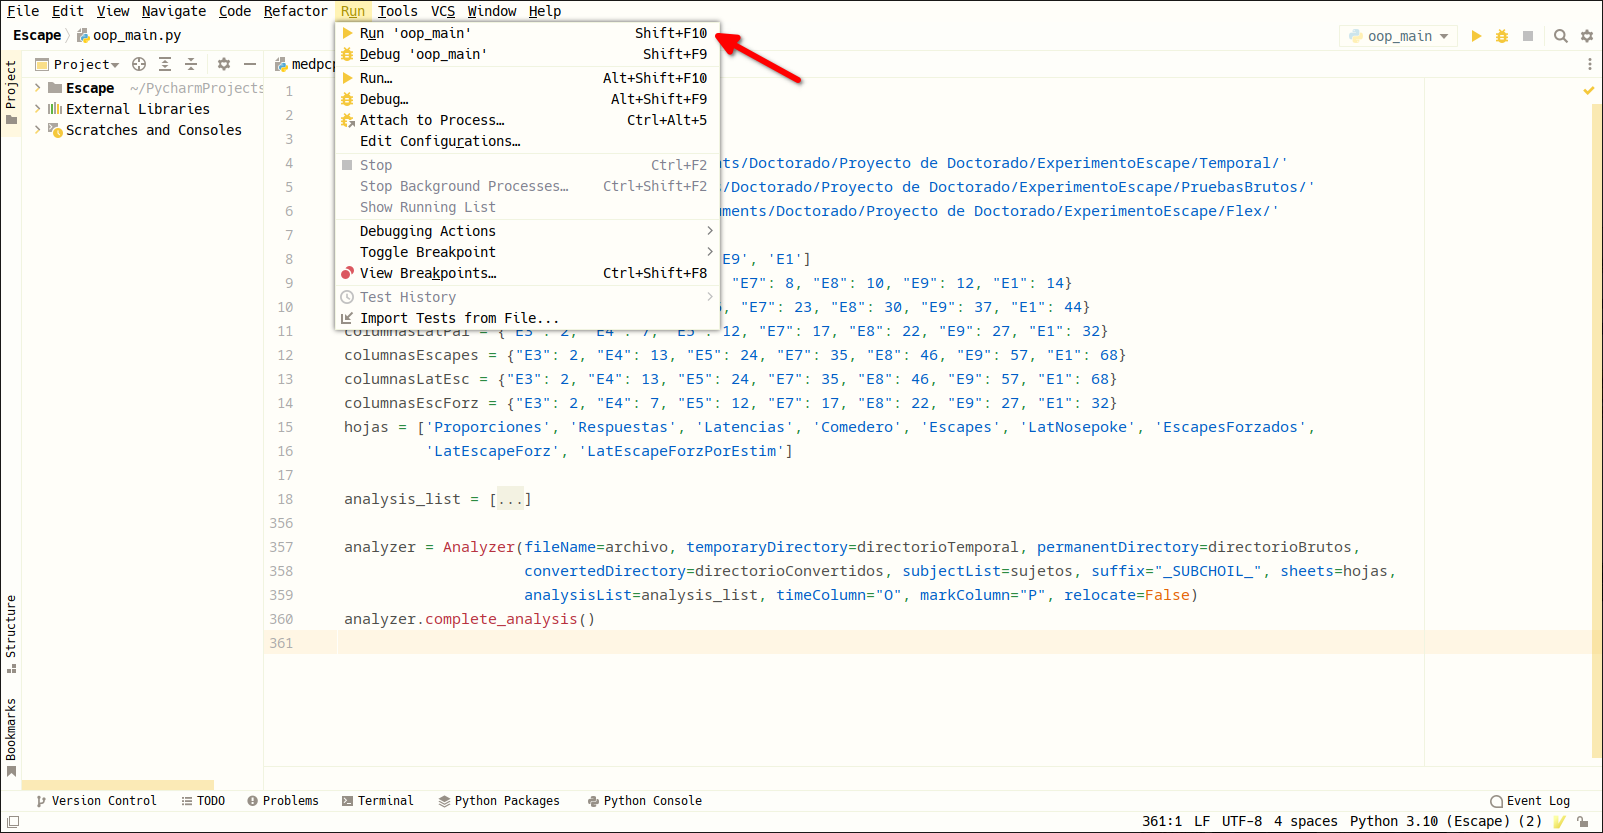
\includegraphics[scale=0.35]{pycharm-run.png}
    \end{center}
\end{figure}

Individual .xlsx files with labeled lists of all declared measures will be created for each session of every subject.

\begin{figure}[!ht]
    \begin{center}
        \includegraphics[scale=0.4]{indiv-file-lists.png}
    \end{center}
\end{figure}

And the summary file will contain central tendency measures. Each session will occupy one row in the summary file, and each column will contain the data for a single measure of a single subject. The labels of the summary file columns seen in the example are not automatically created. Rather, they must be manually written by the user.

\begin{figure}[!ht]
    \begin{center}
        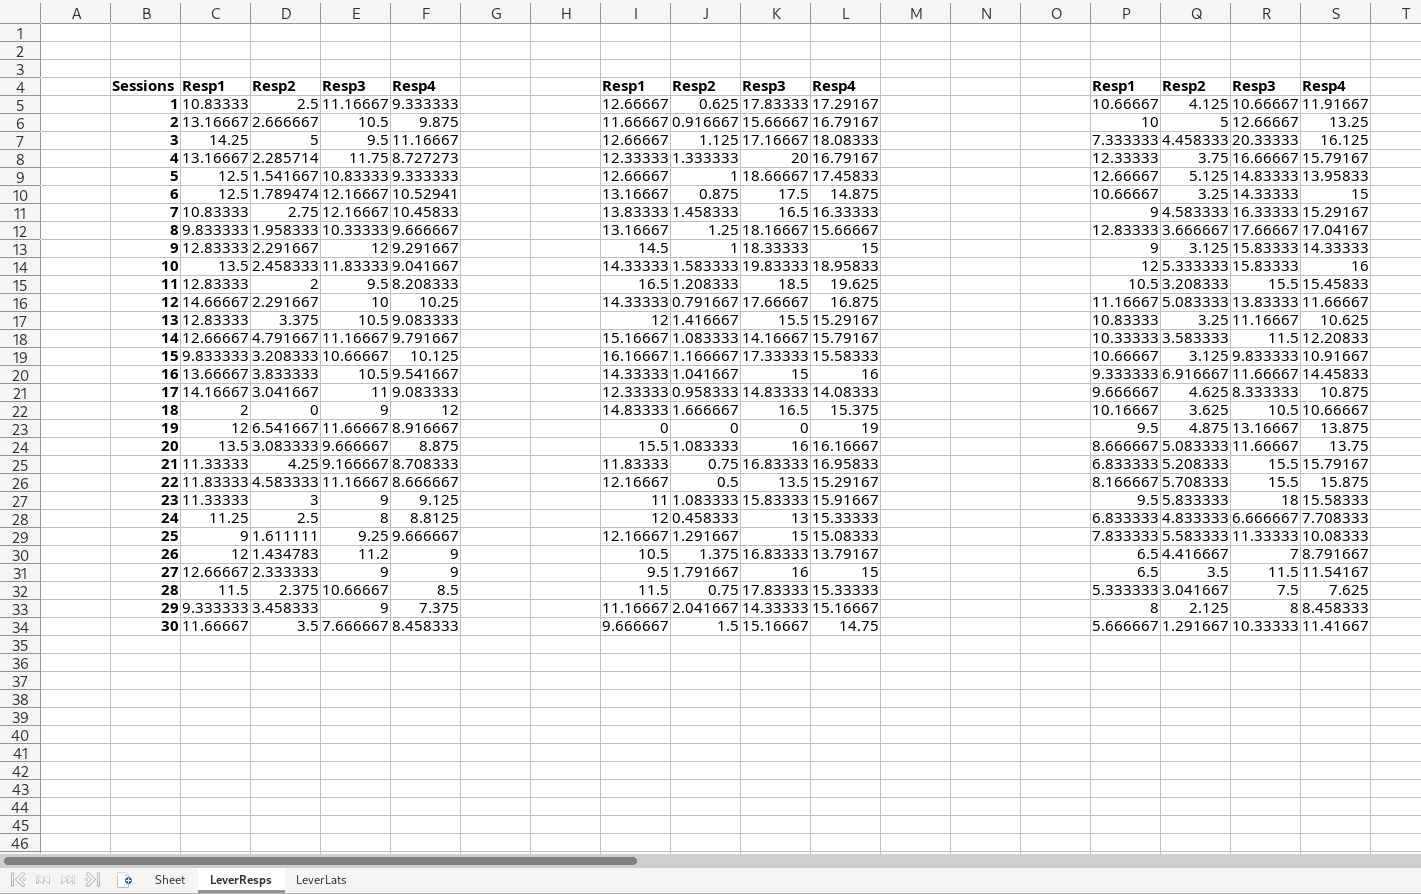
\includegraphics[scale=0.35]{summary-file.png}
    \end{center}
\end{figure}

\newpage
\section{Acknowledgments}

\begin{itemize}
    \item Gabriela E. López-Tolsa, contributor, editor and tester. \href{https://github.com/GELopezTolsa}{Her Github}
\item Rodrigo Uriel González-Torres, contributor, editor and tester. \href{https://github.com/RodrigoUriGT}{His Github.}
\end{itemize}

\section{Other resources}

\begin{itemize}
    \item The official \href{https://www.python.org/doc/}{Python documentation}.
    \item Al Sweigart's \href{https://automatetheboringstuff.com/}{Automate the Boring Stuff with Python}.
    \item Angela Yu's \href{https://www.udemy.com/course/100-days-of-code/}{100 Days of Code}.
\end{itemize}

The team behind MedPCPy is not affiliated with any of these providers. However, their material proved to be useful to develop this library.



\end{document}
